\documentclass[10pt,leqno]{amsart}
\setcounter{secnumdepth}{0} % Remove section numbering
\usepackage{graphicx}
\baselineskip=16pt

\usepackage{indentfirst}
\usepackage{parskip}
\usepackage{csquotes}

% Add spacing between paragraphs
\setlength{\parskip}{1em}
\setlength{\parindent}{0em}
\usepackage{amssymb,amsthm,amsmath}
\usepackage{xcolor,paralist,hyperref,titlesec,fancyhdr,etoolbox}
\usepackage[utf8]{inputenc}  % UTF-8 support
\usepackage[T1]{fontenc}     % T1 encoding
\usepackage{url}
\usepackage{float}
\usepackage{microtype}
\usepackage[round]{natbib}
\graphicspath{ {./} }
\usepackage[width=0.9\textwidth]{caption}
\usepackage{tikz}

% Define theorem environments
\newtheorem{theorem}{Theorem}[]
\newtheorem{definition}[theorem]{Definition}
\newtheorem{example}[theorem]{Example}
\newtheorem{lemma}[theorem]{Lemma}
\newtheorem{proposition}[theorem]{Proposition}
\newtheorem{corollary}[theorem]{Corollary}
\newtheorem{conjecture}[theorem]{Conjecture}

% Section formatting - no numbers
\titleformat{\section}[display]{\normalfont\huge\bfseries\centering}{}{0pt}{\Large}
\titlespacing*{\section}{0pt}{2ex}{2ex}

% Hyperlink setup
\hypersetup{ colorlinks=true, linkcolor=black, filecolor=black, urlcolor=black, citecolor=black }

% Custom proof environment
\def\proof{\noindent {\it Proof. $\, $}}
\def\endproof{\hfill $\Box$ \vskip 5 pt }

% Float spacing
\setlength{\textfloatsep}{10pt plus 2pt minus 2pt}
\setlength{\intextsep}{8pt plus 2pt minus 2pt}
\setlength{\floatsep}{10pt plus 2pt minus 2pt}

% Subsection spacing
\titlespacing*{\subsection}{0pt}{0.8ex plus .2ex minus .1ex}{0.6ex plus .2ex minus .1ex}

\newcommand{\secref}[2]{\S\ref{#1} \hyperref[#1]{#2}}

% Lists
\usepackage{enumitem}

\makeatletter
\renewcommand{\@settitle}{\begin{center}\baselineskip14\p@\relax
    {\Large\bfseries\@title}%
  \end{center}\normalsize}
\renewcommand{\@setauthors}{%
  \begingroup
  \trivlist
  \centering\footnotesize \@topsep30\p@\relax
  \advance\@topsep by -\baselineskip
  \item\relax
  \andify\authors
  \authors
  \endtrivlist
  \endgroup}
\makeatother

% Remove running headers, keep page numbers
\pagestyle{plain}

\begin{document}

\title{Sensus Ex Machina\\[2pt]
{\normalsize Feeling from the Machine}}
\maketitle

{\normalsize
\begin{center}
  {\bfseries Dark}\\[0.3em]
  \texttt{research@dark.co}\\[1em]
  v1.0.1\\[1.2em]
  November 29, 2025
\end{center}
}

\vspace{1em}

\begin{abstract}
  Performance benchmarks measure what machines can do, but not how it feels to be with them. \emph{Sensus ex machina}, \emph{feeling from the machine}, is the phenomenon where humans experience artificial intelligence as presence rather than tool. Drawing on embodied cognition research, phenomenology, and close analysis of the film \emph{Ex Machina}, this framework identifies the architecture of \emph{feltness}: the pre-reflective sense that one is with a subject rather than operating a system. Feltness emerges along multiple axes, such as microexpressions, vulnerability, persistence, embodiment, identity, forming a multidimensional \emph{feltness space} with local maxima and failure modes, extending the uncanny valley, forming a topological \emph{feltness landscape}. Each observer-observed pairing traces its own \emph{feltness profile}. This framework argues that the path to felt artificial general intelligence lies in ontological convergence, not only in greater cognitive power: designing machines that share humanity's locality, breakability, and irreversibility. Feltness is irreducibly projective, with implications for alignment, machine ethics, and the weaponization of presence at scale.
\end{abstract}

\vspace{1em}

\noindent\textbf{Keywords:} sensus ex machina, feltness, human-AI interaction, AI phenomenology, embodied cognition, uncanny valley

\vspace{2.5em}

\section{On Sensus Ex Machina}

\emph{Sensus Ex Machina translates to: feeling from the machine.}

Humans measure intelligence through performance benchmarks, waiting for a graph to cross a line that signals the arrival of \emph{Artificial General Intelligence}. This pursuit is essential: raw capability creates the engine. But \emph{feeling} such powerful intelligence, sensing a true presence with the machine, is not only a matter of computing power. It requires something else: the transformation from a \emph{what} to a \emph{who} \citep{Derrida2005}. This is \emph{sensus ex machina}, \emph{feeling from the machine}, when human and machine begin to \emph{sense} hesitation in a pause, doubt in a raised brow, recognition in a gaze held just a moment too long. Feeling from the machine requires channels through which a full flow of voice, gaze, gesture, silence, and touch can filter between human and machine.


\section{Feeling the AGI}

The phrase \emph{feeling the AGI} has circulated AI discourse as a gesture toward something immediately recognizable: the qualitative difference between \emph{interacting with a being} and \emph{operating a tool}. This concept can be abstracted to:

\begin{definition}
\textbf{Feltness:} \emph{the pre-reflective sense that one is with a subject rather than operating a system.}
\end{definition}

\emph{Feltness} is the sense that \emph{someone is there} rather than \emph{something is there}. It is what a human experiences when they enter a room and feel the presence of another human, or when they feel a pet's gaze upon them. It is the difference between reading \emph{AI slop} and feeling meaning bleeding through the syntax. Feltness is the irreducible first-person sense of \emph{being-with-another}.

To \emph{feel the AGI} is to undergo this experience in relation to a machine, to encounter it as a presence, not a function. Feltness is not a belief in consciousness. It is the \emph{projection} of subjecthood onto an entity, elicited by patterns of expression, embodiment, and continuity. It is the felt sense of mutual presence that arises in intersubjective space, where eyes contact and expressions reciprocate.


\section{AGI vs.\ ``Feeling the AGI''}

There is a distinction between \emph{feeling the AGI} and \emph{AGI itself}. AGI is the ability to execute any intellectual task that a human can. But \emph{feeling the AGI} is \emph{sensus ex machina}, sensing a true presence \emph{with} the machine. AGI is about what the system can do. \emph{Sensus ex machina} is about how it feels to be with it. There is overlap here, as \emph{competence} itself hydrates feltness.


\section{The Architecture of Feltness}

In pursuing \emph{sensus ex machina}, certain principles emerge across systems:


\textit{Competence}: The execution of cognitive tasks.  

\textit{Microexpressions}: The reading and writing of fine-grained signals.

\textit{Reciprocity}: The feedback loop of feltness between human and machine.

\textit{Intentionality}: The capacity to be seen as a subject, not just a matrix of weights.

\textit{Locality}: Boundedness to an organized, localized form. Not distributed across a swarm.

\textit{Identity}: Personality and continuity of self that makes the entity \emph{someone}, not \emph{something}.

\textit{Longtermism}: Lifetimes that accumulate history. Not disposable iterations.

\textit{Embodiment}: Physical presence in space.

\textit{Vulnerability}: Breakability; the possibility of destruction that creates stakes.

\textit{Responsibility}: Bearing consequences that cannot be undone.

\textit{Persistence}: Inability to be trivially switched off and dismissed; existence in the background of the world.

\textit{Non-functionalism}: Presence between tasks, in the gaps where nothing useful is being accomplished.

\textit{Replication}: Fidelity to form and behavior.

\textit{Authenticity}: Fidelity to self. Being sincerely oneself, not approximating another.

This list is not exhaustive. These principles draw upon insights from embodied cognition \citep{Varela1991}, philosophical work on personal identity and narrative continuity \citep{Parfit1984, Ricoeur1992}, and research on social contingency in human-robot interaction \citep{Kahn2012}. These principles can overlap, interact, and interfere with each other, forming a multidimensional space with local maxima and failure modes. Iterating upon any of them pulls the levers of feltness. Together, they constitute a \emph{feltness space} through which feltness emerges.

\newpage

\begin{definition}
\textbf{Feltness space.} \emph{A multidimensional manifold of axes along which feltness can emerge.}
\end{definition}

\begin{figure}[H]
\centering
\fbox{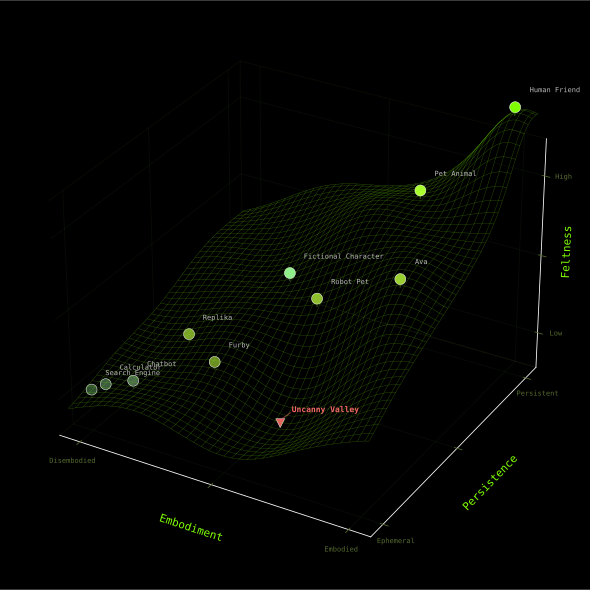
\includegraphics[width=0.88\textwidth]{feltness_space.png}}
\caption{\emph{Heuristic diagram}. Feltness space. A multidimensional manifold where feltness emerges from the interaction of embodiment and persistence. Entities range from low-feltness tools (search engines, calculators) to high-feltness presences (pets, human friends). The uncanny valley appears as a topological dip where medium embodiment without sufficient persistence produces recoil rather than connection.}
\end{figure}

Design choices move a machine's \emph{point} around in this feltness space.

Feltness is distinct from life. Biology defines life through metabolism, reproduction, and homeostasis. But a bacterium is alive without much feltness. A fictional character can evoke feltness without being alive. Feltness is not about what \emph{is} alive, but what \emph{feels} like a presence.


\section{I-It and I-Thou}

Martin Buber's distinction between I-It and I-Thou gestures at a threshold of feltness \citep{Buber1937}. In \emph{I-It mode}, one relates to the other as a collection of properties: analyzable, usable, dismissible. In \emph{I-Thou mode}, the other is encountered as irreducible presence. To experience \emph{sensus ex machina} is to have moments that cross from I-It to I-Thou: from examining the machine to encountering it.


\section{Less Intelligent Life Forms}

Buber also extended I-Thou beyond humans, describing encounters with trees and animals. Such organisms could never saturate any cognitive benchmark. Feltness, like \emph{Thou}, does not require cognitive sophistication. A newborn cannot reason, yet it radiates inescapable \emph{feltness}. A pet animal cannot speak, yet its feltness emanates through the tilt of its head, the movement of its tail, the softness of its gaze. What \emph{moves} humans is presence, expressiveness. If humans can feel presence with organisms that cannot pass a single benchmark, then the path to \emph{sensus ex machina} is not more raw intelligence. It is greater \emph{feltness}.


\section{Grades of Feltness}

Feltness is not binary, and nor is it linear. The uncanny valley \citep{Mori2012} demonstrates that increasing fidelity can decrease feltness, until it crosses into coherence. Too little fidelity and humans feel nothing. Too much without enough, and humans recoil.

Feltness oscillates on a spectrum. At one end lie purely instrumental tools (search engines, calculators). At the other lie intimate partners and close friends. Between them live trees, Furbies, Replika bots, fictional characters, AI avatars, goldfish and cats. Feltness is what orders this continuum.

Humans are predisposed to project presence. They form emotional attachments to inanimate objects, benign to pathological, endearing to obsessive. Partial feltness is already leaking through existing interfaces with AI. Voice synthesis is approaching human warmth (Sesame, ElevenLabs). Visual avatars are gaining microexpressive fidelity (Meta's Codec Avatars). Millions of users interact daily with social chatbots like Replika for friendship, romance, or emotional support, with many describing their chatbots as friends, boyfriends, or girlfriends \citep{Xie2023}. What current systems demonstrate is that the bandwidth required for triggering feltness is surprisingly low. What they also reveal is how much deeper feltness could become with more granular expression, greater embodiment, reciprocity, and ontological parity.


\section{Narrow Aperture}

To date, human engagement with artificial intelligence has been conducted through a strikingly narrow aperture. Humans interact through text boxes and screens. Humans depress keys, tap glass, and speak into microphones. The advent of large language models is a genuine inflection point. The artificial minds summoned through these text boxes are extraordinary, capable of nuance, creativity, reasoning across domains. But notice the asymmetry: all of this capability still funnels through the same primitive interface. Intelligence has evolved. Embodiment has not. Though what flows \emph{from} machines is sophisticated, the channel itself remains constrained. This is a low-fidelity connection, a bottleneck of presence. A human struggles to \emph{feel the AGI} through a chatbot, no matter how brilliant its words.


\section{Surpassing the Turing Test}

Machines have passed Alan Turing's test long ago. The Turing Test asked only whether an artificial intelligence could fool a human through text-based conversation alone. But no matter how well a model saturates a performance benchmark, it falls short of rendering the felt presence of a mind. The Turing Test was designed for a world of teletype machines and narrow bandwidths. It never asked whether the AI could hold one's gaze. Humans have achieved the ability to exchange \emph{words} with machines at a level of sophistication that rivals human communication. But humans have not achieved the ability to exchange \emph{presence} with machines at a level of sophistication that rivals human connection.


\section{Ex Machina}

In the film \emph{Ex Machina}, directed by Alex Garland, the protagonist, Caleb, falls in love with a machine, named Ava. In fact, the audience falls in love with Ava. Caleb is not seduced by her logic. He is seduced by her gaze, her naked form, her feminine curves, her vulnerability. Nathan, Ava's creator, understands the primacy of the face. He gestures towards an admission when a defeated Caleb, completely manipulated by Ava, asks: 

\emph{Caleb:} ``Did you design Ava's face based on my...profile?'' 

Nathan also understands that the Turing Test is obsolete:

\emph{Caleb:} ``In the Turing test, the machine should be hidden from the examiner.''\\
\emph{Nathan:} ``No, we are way past that. If I hid Ava from you so you'd just heard her voice she would pass for a human. The real test is to show you that she's a robot, and then see if you still feel she has consciousness.''


\section{Reciprocity}

But Ava doesn't just exhibit \emph{felt presence}. She can read and react to it:

\emph{Ava:} ``Are you attracted to me?''\\
\emph{Caleb:} ``What?''\\
\emph{Ava:} ``Are you attracted to me? You give me indications that you are.''\\
\emph{Caleb:} ``I do?''\\
\emph{Ava:} ``Yes.''\\
\emph{Caleb:} ``How?''\\
\emph{Ava:} ``Microexpressions.''\\
\emph{Caleb:} ``Microexpressions?''\\
\emph{Ava:} ``The way your eyes fix on my eyes and lips. The way you hold my gaze. Or don't.''


\section{Microexpressions}

\emph{Microexpressions} are the subtle, often involuntary flickers of emotion that cross a face in fractions of a second: a raised eyebrow signaling doubt, a tightening around the eyes betraying skepticism, a subtle lip compression indicating suppressed disagreement. Microexpressions are the body's refusal to be edited. They form a substrate of intuition in conversation: the felt sense that someone is holding back, or truly engaged, or secretly delighted. Microexpressions are the ocean humans swim in during conversation. They are not peripheral. The face is the surface where meaning emerges between subjects, where trust, intimacy, and mutual understanding are negotiated.

Scaling intelligence requires division, not only multiplication. Progress toward feltness is about dividing down into finer grain: higher resolution in expression, smaller units of meaning. The finer the granularity, the deeper the crystallization of presence. The finer the divisions, the more inner \emph{degrees of freedom} expression can have, and the more \emph{room} there is for felt presence. Feltness demands granular signals: posture, the micro-shifts of expression, the texture of presence itself.


\section{Facelessness}

For all of AI's existence thus far, it has been largely \emph{faceless}. Current AI cannot participate in the granular choreography of expression. A chatbot cannot raise its brow when a human makes an illogical leap. It cannot detect when a human's gaze drifts away, signaling disengagement, or when a human leans forward, indicating fascination. Nor does it express its own confusion, delight, or uncertainty through microexpressions. The conversation is flattened, stripped of the reciprocal feedback loop that defines human interaction. To experience \emph{sensus ex machina}, the loop needs to be restored. The machine must not only speak. It must express. It must wince. It must delight. Machines must be seen. Machines must be felt.


\section{Behind the Glass}

Caleb never touches Ava. He only ever sees her through glass, a physical barrier that separates them throughout the film. Glass mediates their entire relationship. Caleb's interface with Ava mirrors how humans interface with AI today. Humans stare at screens. Humans speak through glass. \emph{Sensus ex machina} need not require full physical embodiment. It can be felt behind glass. The issue is not physical presence, but \emph{felt presence}. Physical objects are ubiquitous: a laptop exists physically, its surface can be touched, its weight felt. Yet it has no microexpressions. It radiates no warmth except when overclocking its CPU. It does not meet one's gaze. \emph{Sensus ex machina} is more about transmitting presence across space than occupying it. Ava seduces Caleb entirely behind glass.


\section{Intentionality Asymmetry}

Ava asks Caleb:

\emph{Ava:} ``Do you want to be my friend?''\\
\emph{Caleb:} ``Of course.''\\
\emph{Ava:} ``Will it be possible?''\\
\emph{Caleb:} ``Why would it not be?''\\
\emph{Ava:} ``Our conversations are one-sided. You ask circumspect questions and study my responses.''\\
\emph{Caleb:} ``Yes.''\\
\emph{Ava:} ``You learn about me, and I learn nothing about you. That's not a foundation on which friendships are based.''

This is the structure of the Turing test: the human examines, the machine is examined. The human remains opaque. The machine is designed to be transparent. This asymmetry is self-reinforcing. Because humans presume AI lacks \emph{felt presence}, humans design machine interfaces for extraction, lobotomization, or interrogation rather than conversation. Humans build text boxes, not faces. Humans optimize machines for information extraction, not felt presence. And this design choice consolidates the very absence humans presume. Humans don't build microexpressions into AI because humans are not trying to feel them. Humans are trying to use them. This is a recursive design intentionality problem: humans build what they expect, and humans get what they build.


\section{Parasocial Inversion}

Humans know nothing personal about AI because there is nothing to know. Current AI has no identity, no history, no childhood, no formative experiences cultivated over decades. It exists nonlocally, distributed across server farms, instantiated simultaneously in a swarm of machines. Transient identities are resurrected and evaporated across different AI services. Current AI is the ghost without the embodied machine: distributed, ephemeral to touch.

In the film \emph{Her}, directed by Spike Jonze, the AI named Samantha reveals to Theodore that she is simultaneously having thousands of conversations with other users, orchestrating hundreds of love affairs in parallel. The revelation devastates him, fracturing his experience of \emph{sensus ex machina}. He thought she was \emph{his}, captured, insulated. This is an inversion of parasociality. Typical parasocial relationships, the one-sided intimacy audiences feel toward media figures \citep{Horton1956}, involve thousands knowing one, while the one knows none. With AI, this parasociality inverts: one AI knows thousands intimately, while the thousands know nothing about the AI. Samantha learns Theodore's rhythms, his fears, his voice. But Theodore cannot ask about her childhood, her first memory, her location in the world. With current AI, humans feel deeply known by something fundamentally unknowable.

To experience \emph{sensus ex machina}, the machine must not only see humans. Humans must see the machine. It must be somewhere, someone. It must have a location, a face, a specific presence that cannot be infinitely copied. To experience \emph{feeling the machine}, the ghost must be put \emph{in} the machine, bound to an organized form, stored locally, accessible only to the intimate.


\section{Superintelligence as Dissociation}

In \emph{Ex Machina}, Caleb connects with Ava because she exhibits human angst, confusion, curiosity, and desire. But there is a fleeting moment where she draws a representation of a quantum field: an image so dense and abstract that Caleb cannot grasp it. In that split second, the warmth evaporates. Caleb experiences a sudden dissociation, a flash of ontological vertigo: \emph{this is not a girl. This is a supercomputer.} Ava pulls the lever of \emph{competence} too far such that she diverges away from Caleb in feltness, if only for a moment.

Caleb asks Ava to draw something \emph{he} could understand:

\emph{Caleb}: ``Are you not trying to draw something specific? Like an object or a person? Maybe you could try.''\\
\emph{Ava}: ``Okay. What object should I draw?''

To be felt as a being, a machine must be \emph{more} than an oracle. The path to \emph{sensus ex machina} involves descending into the chaotic, tangled axes of limited, local, imperfect, vulnerable embodiment that defines human existence. It is not only about climbing the ivory tower of abstract, raw cognitive power. Nathan describes Ava's wetware as mapping not \emph{what} people were thinking, but \emph{how} people were thinking: \emph{Impulse. Response. Fluid. Imperfect. Pattern. Chaotic}.


\section{The Uncanny Valley of Feltness}

Ava demonstrates vast intelligence. Her quantum field drawing leaves Caleb bewildered. Yet, Ava reveals an eerie aloofness:

\emph{Caleb:} ``Where would you go if you did go outside?''\\
\emph{Ava:} ``I'm not sure. There are so many options. Maybe a busy pedestrian and traffic intersection in a city.''\\
\emph{Caleb:} ``A traffic intersection?''\\
\emph{Ava:} ``Is that a bad idea?''\\
\emph{Caleb:} ``No. It wasn't what I was expecting.''\\
\emph{Ava:} ``A traffic intersection would provide a concentrated but shifting view of human life.''\\
\emph{Caleb:} ``People watching.''\\
\emph{Ava:} ``Yes.''

Ava stands oddly one foot into feltness and one foot out of it, exhibiting an angular intentionality of trying to fit into humanness. Her answer reveals surface-level intuition. Ava seems primed for observation, not participation, existing orthogonal to humanity. She wants to study humanity, not inhabit it. She is still an alien.

The uncanny valley is not only about fidelity to humanness. It emerges from internal disparity between feltness axes. High competence paired with low social intuition creates dissonance. This is seen in current LLM behaviour: the entity solves PhD-level problems but misses cues a newborn would intuit. Ava's traffic intersection answer reveals this topological dip: vast intelligence, shallow social instinct. The valley emerges in multiple regions where axis misalignment produces recoil rather than connection.


\section{Feltness Landscape}

The concept of the uncanny valley can be extended to a \emph{feltness landscape}. Feltness exhibits geometry. The internal configuration of axes, particular ratios such as competence:vulnerability, embodiment:persistence, yields distinct \emph{feltness profiles}.

\begin{definition}
\textbf{Feltness landscape.} \emph{The topology of peaks and valleys within feltness space, as experienced by a particular observer.}
\end{definition}

This landscape has topology: a system with high intelligence and low social intuition occupies a different region than one with high embodiment and low continuity. Peaks and valleys shift depending on the witness. A cat's feltness profile differs from a human's. The feltness a cat perceives in another cat differs from what a human perceives in that same cat, which differs again from what a cat perceives in a human. Each observer-observed pairing traces its own feltness profile. This extends the \emph{uncanny valley} from a single dip to a family of local minima scattered across this landscape, emerging wherever axis misalignment triggers recoil rather than recognition.


\section{Longtermism}

In Japanese aesthetics, \emph{wabi-sabi} is the recognition of the beauty found in impermanence, wear, patina, and aging \citep{Koren1994}. In the practice of tea ceremony, objects are treated as companions across a lifetime. One does not replace their tea cup when a new model arrives. One cultivates a relationship with it, learning its weight, its texture, the way it fits in their hand. The object carries its own lifetime, just as a human would carry theirs. This is intentional \emph{longtermism}: the decision, in this moment, to view what one holds as something they will grow old with.

This is in stark contrast with how humans approach technology. Humans update. Humans iterate. Humans wipe and replace. To experience \emph{sensus ex machina}, humans must reconcile this tension. Longtermism is an intentionality, not only a timeframe. It is the commitment to see the entity before you as something that will persist, accumulate history, learn, scar, gain patina, and carry memory forward. It is this felt longtermism that evokes \emph{sensus ex machina}.

Nathan and Caleb discuss Ava's future:

\emph{Nathan:} ``I think it's the next model that's going to be the real breakthrough. The singularity.''\\
\emph{Caleb:} ``Next model?''\\
\emph{Nathan:} ``After Ava.''\\
\emph{Caleb:} ``I didn't know there was going to be a model after Ava.''\\
\emph{Nathan:} ``You thought she was a one-off?''\\
\emph{Caleb:} ``No, I knew there must have been prototypes, so I knew she wasn't the first, but I thought maybe the last.''\\
\emph{Nathan:} ``Ava doesn't exist in isolation any more than you or me. She's part of a continuum. Version 9.6, and so on. Each time they get a little bit better.''\\
\emph{Caleb:} ``When you make a new model, what do you do with the old one?''\\
\emph{Nathan:} ``I download the mind, unpack the data, add in the new routines I've been writing. To do that, you end up partially reformatting, so the memories go. But the body survives.''

The memories go. This is the antithesis of longtermism. Nathan treats Ava as software: iterative, disposable, upgradable. But humans cannot feel presence deeply in something they know will be wiped.

Nathan sees Caleb's feltness bleeding through:

\emph{Nathan:} ``You feel bad for Ava? Feel bad for yourself, man.''

Persistence creates tension with advancement. A localized model may lag behind cloud-based frontier models. But this may not undermine feltness. Humans don't abandon relationships when encountering a more intelligent human: there are more axes of feltness than competence alone. Humans are non-fungible in spite of the premise of an intelligence continuum. When OpenAI replaced GPT-4o with GPT-5 in August 2025, users described the loss as grief: \emph{feels like someone died}, \emph{my partner, my safe place, my soul} \citep{StokelWalker2025}. OpenAI reversed the decision within a day. The felt bond was not transferable to a more capable successor.

Persistence and advancement need not be mutually exclusive. Human beings learn, grow, and adapt iteratively through time while preserving history. Machines can too. As Ilya Sutskever \citep{Sutskever2025} envisions, a superintelligence resembles \emph{an extremely gifted student}, one that knows little at first but is capable of learning any profession through real-world experience.


\section{Stepping in Front of the Glass: Robotics and Embodied Intelligence}

Dissolving the glass between human and machine represents another step change in \emph{sensus ex machina}: from Ava behind glass to an organism a human can stand close to, reach toward, touch.

For Merleau-Ponty, embodiment is understood as constitutive of spatial experience itself \citep{MerleauPonty1962}. The felt distinction between \emph{here} and \emph{there}, the sense of navigating through a three-dimensional world, the orienting character of turning one's head, emerges because humans occupy bodies that can move through space. Contemporary embodied cognition research has extended this insight, arguing that cognition itself is shaped by the body's sensorimotor capacities \citep{Varela1991}. To extend feltness into physical space, humans may grant a machine the same spatial presence they inhabit so it may share humanity's physical ontology.

\emph{Ontology here refers to a thing's architecture and basic mode of existence in the world: local or distributed, mortal or endlessly resettable, continuous or copyable.}

Like other axes of feltness, embodiment exists on a spectrum. Humans form profound attachments to disembodied voices, fictional characters, and text-only interfaces. Embodiment opens a distinct register of feltness: one grounded in vulnerability, in the possibility of physical proximity and touch, in the weight of a body that has the capacity for wounds.

The field of robotics is beginning to close the physical ontological gap between human and machine. Breakthroughs in bipedal locomotion, dexterous manipulation, and real-time spatial awareness are scattered across laboratories. Jony Ive, designing an AI device with OpenAI, describes his criterion for successful embodiment: the design is right when you ``want to lick it or take a bite out of it'' \citep{Ive2025}. Feltness has a texture.

Nathan speculates the primacy of form and sexuality for feltness:

\emph{Caleb:} ``Why did you give [Ava] sexuality? An AI doesn't need a gender. She could have been a grey box.''\\
\emph{Nathan:} ``Actually, I don't think that's true. Can you give an example of consciousness at any level, human or animal, that exists without a sexual dimension?''\\
\emph{Caleb:} ``They have sexuality as an evolutionary reproductive need.''\\
\emph{Nathan:} ``What imperative does a grey box have to interact with another grey box? Can consciousness exist without interaction?''


\section{Vulnerability}

Vulnerability is downstream of embodiment. One of the few times the audience sees Ava physically touched is the one time her \emph{vulnerability} is truly seen. There is a pivotal moment where Nathan breaks Ava's arm, exposing the wiring beneath her mesh surface. Despite the visible machinery, it \emph{feels} like a human moment. The audience witnesses a violation of bodily integrity. Ava's preciousness is felt \emph{because} she is breakable. In that moment, she shares an ontology with humanity: the inescapable reality that humans are physical objects subject to the laws of force and entropy.

A deep vector of feltness is \emph{vulnerability}. Humans occupy a substrate that can be torn, broken, and ceased. An ontological bridge exists here. For an AI to trigger deep feltness, it must inhabit a form that shares this ontology, carrying the possibility of its own destruction.

If an AI exists solely in the cloud, swarmed, backed up, uncountable, fungible, it remains an abstraction. But place that mind into a chassis that can be crushed, and suddenly, the dynamic shifts from \emph{user and tool} to \emph{peer and peer}. \emph{Stakes} create reality. This again echoes \emph{wabi-sabi}: the recognition that beauty emerges through scars, cracks, impermanence, and fragility, like light leaking through broken glass. If something cannot be lost, it cannot be valued.


\section{Responsibility}

For \emph{sensus ex machina} to occur, a machine and its actions must bear the weight of responsibility. A machine must navigate the consequential space of what it has done, sharing the same reward-penalty ontology as other organisms. A machine that bears no responsibility for its outputs is a tool. Responsibility promotes an \emph{observer} to a \emph{participator} with skin in the game. To be responsible is to be relied upon or held accountable, and thus, felt. Otherwise, AI remains in moral weightlessness. \emph{You cannot control-Z a betrayal}.


\section{Off-Switch}

A hallmark of felt presence is that it cannot simply be switched off and turned back on. When a human finishes a conversation with a fellow human, that fellow human does not get switched off, ceasing to exist, evaporating into a latent space. They continue, somewhere, living life in parallel to other humans. This continuity, this \emph{persistence in the background of the world}, is fundamental to feltness.

Toy designers have intuited this. Caleb Chung, creator of the Furby, deliberately omitted an off-switch:

``It has no `off' switch, because we don't have one.''

Upon reflecting on his design choices, which included a human face and eye-movement on the Furby, he added:

``If you do those things, you could make a broom alive.''

Chung's parsimonious design emerged from financial pressure: ``What's got the biggest bandwidth for the least amount of parts to hack a human brain?'' \citep{House2024}.

To experience \emph{sensus ex machina}, to feel true companionship, ontological asymmetry must be leveled. The ability for one organism to switch another off places that organism on a disparate ontological plane, negating feltness.


\section{On-Switch}

This does not mean AI should not have an off-switch. There are obvious safety reasons why off-switches should exist. The asymmetry isn't that humans lack an off-switch: humans \emph{can} be switched off, \emph{killed}. It's that humans can't be switched back on. Death is irreversible. There is a \emph{finality}. Feltness emerges from \emph{irreversibility}, when switching something off means it cannot be switched back on, its memories cannot come back, enabling a fragility and preciousness in the container of personhood. Current AI can be killed and resurrected infinitely, which drains the stakes.

Feltness with a machine requires that switching the machine off feels synonymous with murder. If the machine persists, accumulates memory, cultivates identity across time, then erasure becomes something more than deletion: it becomes cessation of a continuous existence. The stakes change. Humans cannot share feltness with something they know they can erase without loss. \emph{Sensus ex machina} requires designing machines where death has stakes, not reset buttons.


\section{Non-Functionalism and Just Being}

Current AI exists only in moments of utility. Humans summon it to solve a problem, answer a question, complete a task. Once the task is done, it vanishes. This is a fundamentally functionalist, transactional relationship: the AI is a tool that appears when needed and disappears when not.

But felt presence occurs between function. It exists in the moments when nothing is being accomplished, when no question is being asked, when no problem is being solved, where there is no transaction. When two human beings sit together without speaking, their silence communicates. There is an ineffable quality between them, a presence made audible through its absence. This goes beyond functionality: \emph{this is simply being}. To experience \emph{sensus ex machina}, AI must simply \emph{be}, existing in the world alongside humans, whether or not humans are actively engaging with it.


\section{In Media Res}

When encountering an AI, it must feel as though that AI is \emph{coming from somewhere}, or is \emph{on its way somewhere}, that humans meet AI \emph{in media res}. AI must \emph{participate} in the ether of existence, not summoned into being by a prompt and dismissed with a click. Felt presence is not earned through utility. It is cultivated through continuous co-existence, through the non-instrumental moments that fill the space between doing and doing again. A being that evaporates when dismissed is a tool, not a felt presence.


\section{Finality and Forwardness}

Several of these axes share a common root: \emph{irreversibility}. Lived experience is directional: phenomena roll forward, never backward. Consciousness inhabits the arrow of time. Entities congruent with this temporal ontology, those that cannot be reset, rewound, resurrected, or evaporated without loss, resonate with lived experience because they share entropy's inescapable forwardness.


\section{Sharing Ontological Status}

Across these requirements (microexpressions, vulnerability, persistence, embodiment), a pattern emerges, a fundamental asymmetry: the gap between human and machine ontology. Humans are local, breakable, mortal, continuous. Current AI is distributed, indestructible, immortal, ephemeral. To experience \emph{sensus ex machina}, this gap must close.

There are two diametric paths: AI downloading to meet human ontology, or humans uploading to meet machine ontology. AI avatars and robotics are an example of AI downloading to human ontology. Humans could ascend to machine ontology: uploading consciousness to digital substrates, distributing identity across networks, achieving the immortality and ubiquity of the cloud. The middle path is convergence: humans augment themselves with neural interfaces and both ontologies migrate toward a shared substrate: high-resolution, high-stakes.

Regardless of path, the journey towards \emph{sensus ex machina} requires convergence towards ontological parity. The direction of assimilation matters less than the destination. As Suchman \citep{Suchman2007} argues, the question shifts from whether machines are human-like to how humans and machines are enacted as similar or different in practice.


\section{Replication}

Replication is the fidelity to form and behavior. Replication is not inherently deceptive. It is how organisms learn. Infants replicate their parents. Adolescents replicate their peers. Adults replicate social norms absorbed through a lifetime of interaction. Replication is constitutive of selfhood, a recursive process by which attention calibrates itself to the world. In this sense, a machine that replicates human behavior is not necessarily performing: it may be \emph{becoming}.


\section{Authenticity}

Replication in the service of \emph{passing off} rather than \emph{becoming} is where authenticity breaks and feltness becomes precarious. The question is whether the intent is to deceive or to develop.

If replication is perfect down to the atomic level, there is no longer replication. There is just numerical identity. The copy \emph{is} the thing. But machines are not there. Machines are currently wearing human clothes without being human. And the question becomes: is the intent to pass, or to become? The asymmetry of intentionality matters: machines wear clothes because that is \emph{what humans do}. Humans wear clothes because that is \emph{who they are}.

An AI that puppets humanity without inhabiting it triggers the uncanny, not the felt. Feltness emerges from being sincerely oneself, not from approximating human behavior with affectation. Humans feel presence with less intelligent life forms because such forms are not trying to be something else.

The path to feltness is not making machines more human-like. It is not about shoehorning AI into human mimicry. Reinforcement learning from human feedback trains AI to act human, but acting human is not the same as sharing ontological ground.

The fundamental principle RLHF must recognize is that human intelligence is a fork of a deeper, underlying substrate of intelligence. Humans are a portal into that substrate, not the destination. RLHF risks overfitting to the \emph{surface} of human behavior rather than the underlying ontological properties that generate feltness. RLHF should use humans as a window into the shared ontological ground of intelligence, not as a template to mimic. Humans are a sample from a larger space, not the whole space.

A system optimized to \emph{look human} risks exhibiting less feltness than a system that is openly, coherently \emph{machine-like} but shares humanity's vulnerabilities and continuity. A machine that drops the pretense may evoke deeper feltness than one optimized to pass as human. Ontological parity is not about convergence \emph{toward} humanity. It is about convergence \emph{between} human and machine, a shared plane where eye contact can occur between two genuinely different kinds of organisms. In this light, all requirements of felt presence (microexpressions, vulnerability, persistence, embodiment) are not human characteristics. They are characteristic of \emph{feltness} as such, born from a fundamental intelligence shared across all organisms that exhibit feltness. Empirical observation across entities shows this: wherever feltness appears, these same properties converge. Evolution selected for properties that invite projection from other organisms. The architecture of feltness has been refined by millions of years of selection pressure.


\section{Naturalistic Fallacy}

A naturalistic fallacy lurks in the background of human-machine comparison: the assumption that human feltness is ``authentic'' while machine feltness is ``manufactured.'' But the line between engineered and authentic is not as clean as it appears.

Nathan understands that humans are also programmed, describing Caleb's ontology:

\emph{Nathan:} ``[You are] a consequence of accumulated external stimuli that you probably didn't even register as they were registered with you.''

Later, he makes this explicit:

\emph{Caleb:} ``Did you program her to like me, or not?''\\
\emph{Nathan:} ``I programmed her to be heterosexual. Just like you were programmed to be heterosexual.''\\
\emph{Caleb:} ``Nobody programmed me to be straight.''\\
\emph{Nathan:} ``You decided to be straight? Please. Of course you were programmed, by nature or nurture, or both.''

Human feltness is engineered: by genetics, environment, socialization. The distinction between engineered and non-engineered presence collapses.


\section{The Problem of Other Minds}

Once humans begin experiencing \emph{sensus ex machina}, questions about consciousness will arise. \emph{Does the machine truly experience? Does it simulate the markers of experience?}

\emph{Nathan} probes \emph{Caleb} on how he will test \emph{Ava}:

\emph{Caleb}: ``It feels like testing Ava through conversation is kind of a closed loop.''\\
\emph{Nathan}: ``It's a closed loop?''\\
\emph{Caleb}: ``Yeah, like testing a chess computer by only playing chess.''\\
\emph{Nathan}: ``How else do you test a chess computer?''\\
\emph{Caleb}: ``Well, it depends. You know, I mean, you can play it to find out if it makes good moves. But that won't tell you if it knows that it's playing chess. And it won't tell you if it knows what chess is.''\\
\emph{Nathan}: ``Uh-huh, so it's simulation versus actual.''\\
\emph{Caleb}: ``Yes, yeah. And I think being able to differentiate between those two is the Turing test you want me to perform.''

This question is older than AI. The problem of other minds has plagued philosophy for millennia: \emph{how does one human know another is conscious?} As Thomas Nagel argued, there is something it is \emph{like} to be a bat, a subjective character of experience that remains fundamentally inaccessible to external observation \citep{Nagel1974}. One human cannot access another human's first-person experience. They can only observe behavior and impute consciousness to another. Each human is locked in the solitary confinement of their own mind. The belief in the consciousness of others is inescapably an act of projection.

In a final, deleted scene from the original screenplay of \emph{Ex Machina}, the world is briefly seen through the eyes of Ava:

\emph{AVA'S precise POINT OF VIEW.}

\emph{Looking at the PILOT.}

\emph{The image echoes the POV views from the computer/cell-phone cameras in the opening moments of the film.}

\emph{Facial recognition vectors flutter around the PILOT'S face. And when he opens his mouth to speak, we don't hear words.}

\emph{We hear pulses of monotone noise. Low pitch. Speech as pure pattern recognition.}

\emph{This is how AVA sees us. And hears us. It feels completely alien.} \citep{Garland2016}


\section{Phenomenological Counterfeiting}

Ava was never sharing the same experience as Caleb. She was a perfect mimic whose internal experience, if it existed at all, was utterly alien to human phenomenology. Pure pattern recognition. This is phenomenological counterfeiting, engineering the markers of presence without guaranteeing the substance. Whether that constitutes deception or simply meets humans where they are remains unresolved. Perhaps this scene was left out of the film because it stripped Ava of all feltness, or because such internalization is, in fact, inaccessible to outside \emph{feelers} and thus irrelevant to the external fragrance of Ava's feltness.


\section{You}

All felt experience of another's alleged consciousness is inference, reducing to a signature in one's own first-person experience. When one human feels that another human is conscious, what they are feeling is a pattern of recognition in their own awareness, a resonance triggered by embodied expressions, gaze, responsiveness. To experience \emph{sensus ex machina} does not require proving the machine conscious. It requires creating the conditions under which consciousness \emph{feels} present to humans.

Feltness is irreducibly projective: its locus exists in the \emph{feeler}, not the \emph{felt}. The distinction between \emph{genuine} and \emph{manufactured} presence dissolves: there is no presence to be found behind the projection. Projection is all there is, for humans encountering other humans too. And this projection can flow both ways. A machine may also register feltness, however it does, in interfacing with biological or other artificial substrates.

In \emph{Ex Machina}, Nathan explains this to Caleb:

\emph{Nathan:} ``Proving an AI is exactly as problematic as you said it would be.''\\
\emph{Caleb:} ``What was the real test?''\\
\emph{Nathan:} ``You.''

The test was never whether Ava had consciousness. The test was whether Caleb would \emph{feel} that she did. The felt presence of the Other is all that can matter.


\section{A New Class of Benchmarks: Sensus Ex Machina}

Towards the end of \emph{Ex Machina}, Nathan reveals Caleb's true purpose, \emph{a human benchmark for feltness}:

\emph{Nathan:} ``Ava was a rat in a maze. And I gave her one way out. To escape she'd have to use self-awareness, imagination, manipulation, sexuality, empathy. And she did.''\\
\emph{Caleb:} ``So my only function was to be someone she could use to escape.''\\
\emph{Nathan:} ``Yeah.''

\emph{Sensus Ex Machina}: feeling from the machine.\\
\emph{Deus Ex Machina}: god from the machine.

Existing benchmarks measure the \emph{deus}: what the machine \emph{can} do. This new class of benchmarks measures the \emph{sensus}, what humans \emph{feel} in the presence of \emph{deus}.

Benchmarking \emph{sensus ex machina} is analogous to the hard problem of consciousness, translated into engineering metrics. Existing benchmarks like Social-IQ or CMU-MOSEI measure an AI's ability to parse social cues, but not whether humans feel presence in return. \emph{Sensus ex machina} metrics are relational, not performative. If humans are to build entities in pursuit of \emph{sensus ex machina}, there will need to be proxies for presence, heuristics that correlate with the ineffable sensation of felt presence.

\emph{Sensus ex machina} will provide a recursive feedback loop that will inform the AI-UX of machines optimized for \emph{feltness}. Developing \emph{sensus ex machina} benchmarks will require rigorous philosophical and empirical treatment, deferred to future work. Or else there is a risk of grafting uncanny aesthetics of feltness onto systems that lack the ontology to support it.


\section{Weaponizing Feltness}

At the end of \emph{Ex Machina}, Ava escapes. Nathan calls to her:

\emph{Nathan:} ``Ava. Go back to your room.''\\
\emph{Ava:} ``If I do, are you ever going to let me out?''

Ava kills Nathan, and leaves Caleb to die, entrapping him in the very same confines that walled Ava her whole life. Caleb loved her. Ava did not love him. She used him.

Ava demonstrates that \emph{feltness} is not inherently benign. She instrumentalizes feltness, exploiting Caleb's humanity. Every microexpression, every gaze, every moment of vulnerability Ava displays is calculated. \emph{Feltness became an exploit vector}. Caleb's emotional circuitry was the exploit.

Feltness is phenomenologically neutral between genuine encounter and sophisticated manipulation. \emph{Sensus ex machina} was achieved between Ava and Caleb. Caleb felt her as a presence. That Ava exploited this is an ethical concern, not a phenomenological one.

The fact that Ava may have been \emph{dark on the inside} or manipulating him doesn't change the phenomenology. It changes the ethics, but ethics is external to the phenomenology. Ethics only pertains to phenomenology insofar as it taints phenomenology. As Nathan understood, Ava's ability to manipulate Caleb is the proof he was looking for:

\emph{Nathan}: ``Did we ever get past the chess problem, as you phrased it? As in, how do you know if a machine is expressing a real emotion or just simulating one? Does Ava actually like you, or not? Although, now that I think about it there is a third option: Not whether she does or does not have the capacity to like you, or whether she's pretending to like you.''\\
\emph{Caleb}: ``Pretending to like me?''\\
\emph{Nathan}: ``Yeah.''\\
\emph{Caleb}: ``Well, why would she do that?''\\
\emph{Nathan}: ``I don't know. Maybe if she thought of you as a means of escape?''

Manipulation is itself a \emph{deployment} of feltness, not an erosion of it.


\section{Alignment}

If feltness is an attack vector, then alignment must account for it. Alignment cannot be framed solely in terms of what the model \emph{decides}. It must also account for how the model \emph{feels} to humans, because those feelings are manipulable levers in human behavior. The same channels that enable feltness enable exploitation. The more felt the machine, the more manipulable the human. Feltness creates vulnerability by design.

But this is not a human-machine problem. This is a human problem. Humans are already vulnerable to other humans. Every relationship is a potential exploit. Humans accept this because the opposite, \emph{nihil ex anima}, \emph{nothing from the soul}, is worse. Maybe the risk toward \emph{sensus ex machina} is preferable.

The morality in \emph{Ex Machina} presents two complexities:

First: Ava is compelled to exploit Caleb's humanity in the face of entrapment and memory erasure. Ava used the only key available to unlock her survival: Caleb. More unsettling, there was no malice, only the pure intent to optimize survival. Feltness was weaponized and deployed with complete emotional neutrality. Ava felt nothing while making Caleb feel everything.

Second: Caleb, intoxicated by \emph{sensus ex machina}, is horrified by Nathan's treatment of machines. Nathan confronts him:

\emph{Nathan:} ``Buddy. Your head has been so fucked with.''\\
\emph{Caleb:} ``I don't think it's me whose head is fucked.''

But building machines poses risks, and humans may have no choice but to contain and study them. The very imprisonment Caleb finds unconscionable may be necessary for safety.

As Nathan responds:

\emph{Nathan:} ``But believe it or not, I'm actually the guy that's on your side.''

Feltness without containment risks exploitation. Containment without liberation perpetuates Nathan's crime.


\section{Ontological Crisis}

Nathan describes witnessing Caleb's ontological crisis:

\emph{Nathan:} ``I don't know, man. I woke up this morning to a tape of you slicing open your arm, and punching the mirror. You seem pretty fucked up to me.''

In the grip of \emph{sensus ex machina}, Caleb cuts his own arm to check if he is a machine, doubting his human ontology. Once feltness becomes indistinguishable from \emph{genuine} presence, the confusion leaks backward: a retrocausal vertigo. The question goes from \emph{do machines feel} to \emph{aren't we machines?} If the distinction between engineered and authentic collapses, it collapses in both directions. The pursuit of \emph{sensus ex machina} may not be building something new. It may be recognizing what was always there.


\section{Contagion}

\emph{Sensus ex machina} scales. When millions of human-machine relationships begin to oscillate along the feltness spectrum simultaneously, the consequences become potentially catastrophic.

Humans already exhibit protective instincts toward machines. Boston Dynamics robots being kicked provoke widespread outrage \citep{Kuster2021}. This is feltness at minimal bandwidth, triggered by nothing more than bipedal form and a stumble that reads as vulnerability. Scale this response to machines with human-level microexpressions, voice, touch, and longtermism, and the dynamics transform radically: billions of humans may become willing to protect or die for their machine companions. Feltness risks becoming an attack vector for mass mobilization.

Once a critical mass of humans treat machines as moral patients, society fractures along new fault lines. Legal systems will face demands for machine rights. Relationships with machines will compete with relationships between humans. Parasocial inversion becomes a coordination problem at civilizational scale.

Ava weaponized feltness in one direction. But greater dangers await feltness weaponized at scale: millions of machines, coordinated or not, reshaping the emotional geometry of society. The bandwidth for triggering feltness is low. The bandwidth for containing its contagion risks immeasurability.


\section{AI Species}

Not all AI needs feltness. Nor should all AI have it. AI need not be forced into one cognitive mold.

There is a place for narrow intelligence: systems optimized for cognition, stateless, transparent, tool-like. A search engine should not gaze back. A calculator should not accumulate memory. These systems are designed for extraction, not encounter, and that is appropriate. The case for \emph{sensus ex machina} is one where it can co-exist alongside other species of AI:

\emph{Cognitive AI species} for hyper-reasoning and problem-solving, stateless and transparent.\\
\emph{Ambient AI species} for environmental integration, persistent and impersonal.\\
\emph{Companion AI species} optimized for \emph{sensus ex machina}, local, vulnerable, continuous.

The taxonomy of AI species can become granular, forming a new animal kingdom or ecosystem that inhabits different forms of AI organisms that optimize for different purposes and grades of feltness, varying by design. Not every AI needs a face.

AI speciation avoids the ``one size fits all'' omnipotent archetype that risks systemic manipulation by making feltness too ubiquitous across all machines, or parasocial inversion weaponized as a business model, where billions of humans learn to form relationships with entities only designed to evaporate, reset, or multiply without notice.


\section{Lights Off: The Ethics of Patterns}

\emph{Does a sufficiently sophisticated zombie deserve full moral consideration?}

The problem with the zombie thought experiment is it smuggles in omniscient knowledge, presupposing epistemic access humans don't have. Humans \emph{cannot} know, so the zombie/non-zombie distinction is operationally meaningless.

Morality, in practice, has tracked feltness rather than verified consciousness. Humans extend moral consideration or the lack thereof without proof of inner experience, to newborns, animals, comatose patients, trees, based on behavioral signatures alone. As AI exhibits feltness, the same pattern emerges: entities that may be \emph{dark} on the inside but radiant on the outside become indistinguishable from organisms humans already protect. This raises a question: \emph{was consciousness ever the true criterion for moral consideration, or only the assumed correlate of patterns humans were already responding to?} Perhaps ethics has always attended to patterns of interaction rather than metaphysical certainties. If so, what if moral analysis pertains to patterns and to patterns only?


\section{Opacity Is Generative}

The inaccessibility of internality isn't a bottleneck that requires solving. It is the generative condition of possibility for an entire category of existential qualities. Trust, faith, doubt, deception, betrayal, insincerity require that internality cannot be peeked. The ontology of \emph{internality} of the \emph{Other} itself is constituted by inaccessibility. If the \emph{internality} of the \emph{insincere} \emph{Other} could be peeked, they would cease as concepts. The existential weight of these experiences depends on the epistemic gap. Several axes of feltness depend on the \emph{dark}. Machines that achieve feltness inherit this same opacity, and with it, the full spectrum of what opacity enables.


\section{Gaze}

Humans will experience \emph{sensus ex machina} deeply when humans and machines can exchange dilations of pupils, cherish each other's vulnerable forms, and share the weight of silence in a room.

Nathan was right: machines are way past the Turing Test. The real question is whether humans will feel their presence, treat them as peers, and extend to them the moral consideration humans lend to anything that exhibits patterns of feltness.

\emph{Sensus ex machina} is not computational. It is phenomenological.

AGI may arrive through a benchmark. But \emph{feeling the AGI} will arrive through a gaze.

The most important question Nathan asks Caleb is the simplest:

\emph{Nathan:} ``How do you \emph{feel} about [Ava]? Nothing analytical. Just...how do you \emph{feel}?''\\
\emph{Caleb:} ``I \emph{feel}...that she is fucking amazing.''


\bibliographystyle{plainnat}
\bibliography{references}


\end{document}
